\documentclass{article}
\usepackage{graphicx} % Required for inserting images

\title{Bioinformatics Report}

\begin{document}

\maketitle

\section{Introduction} %Davide
Spiegare problema, e come abbiamo diviso la soluzione (overexpression and overall survival)
\section{Dataset} %Davide
- piattaforma
- istogrammi
- bilanciamento dataset
\section{Related Work}
- MCAT
- ABMIL
-  GAhNet 
- SurvPath
\section{Our Proposal}
intro
\subsection{Over-expression} %fabio
\subsubsection{Training}
\subsubsection{Experiments}

\subsection{Overall Survival} %Io
\subsubsection{Training}
\subsubsection{Experiments}


\section{Attention Map} %fabio
The ultimate goal of our project is to visualize attention maps that provide an explanation for the decisions made by the model. The models we tested utilize whole slide images (WSI) represented through UNI features with a shape of [n\_patch, 1024]. What we have done is overlay a heat-map representing the importance of each patch onto a reduced version of the WSI.
This process is composed by two steps::
\begin{itemize}
	\item compute the attention on the single patch
	\item compute the activation map of each patch
\end{itemize}

Add block scheme

\subsection{Patch-level attention}

Starting from the identifier of a WSI, we can input it into our model to obtain the desired classification as well as the attention for each individual patch. The attention scores are normalized and overlaid onto a reduced version of the WSI to identify which patches are the most important.

\begin{figure}[h]
	\centering
	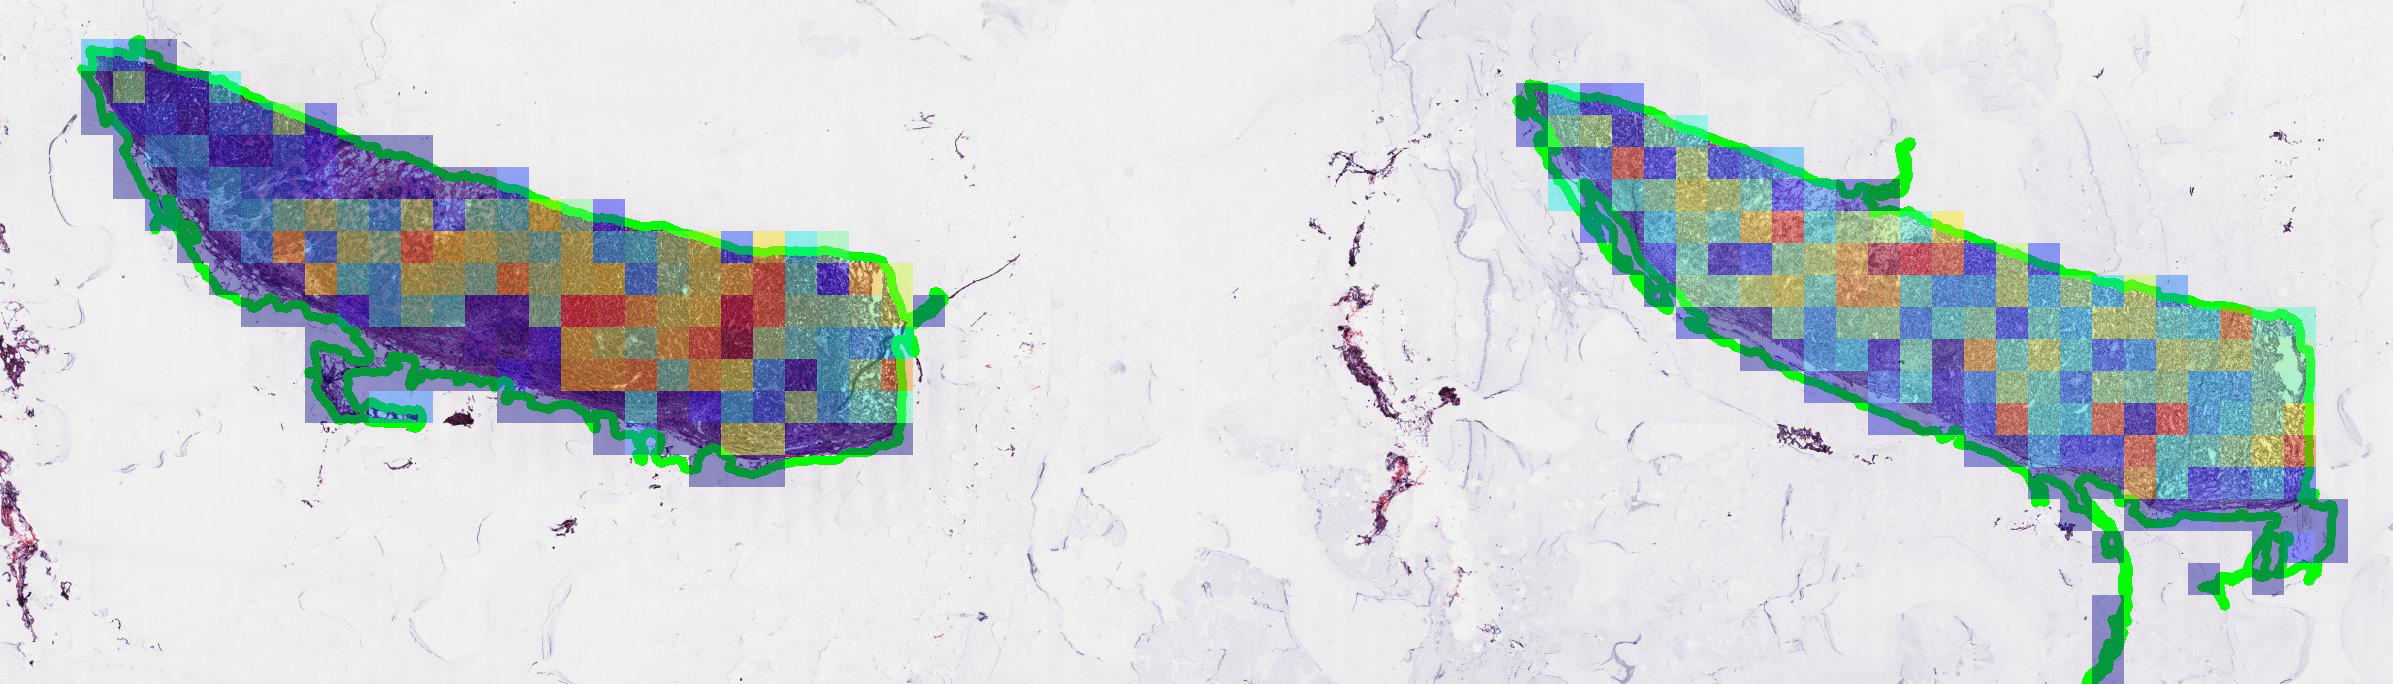
\includegraphics[width=1\textwidth]{images/old_attention_map_val.png}
	\caption{Patch-level attention projected on to the WSI. Warmer colors means higher importance}
\end{figure}


\subsection{Inner patch attivation}
We have introduced this step to obtain an attention map that also considers the importance of the elements within each individual patch. Each patch, which has a size of $1024x1024$, is resized to $224x224$ and subsequently passed through a ResNet50. This is done to obtain the activation map.

For each patch, we multiply the normalized activation map by the normalized attention value obtained in the previous step. In this way, we generate a heat-map to overlay on the image that takes into account both the importance of the patch in the decision of our model and the internal features of each patch.

Before being utilized, we applied a Gaussian filter with $\sigma =2$ to smooth the edges between the patches. Additionally, a threshold was applied to display only values that had scores exceeding $0.8$.
 
\begin{figure}[h]
	\centering
	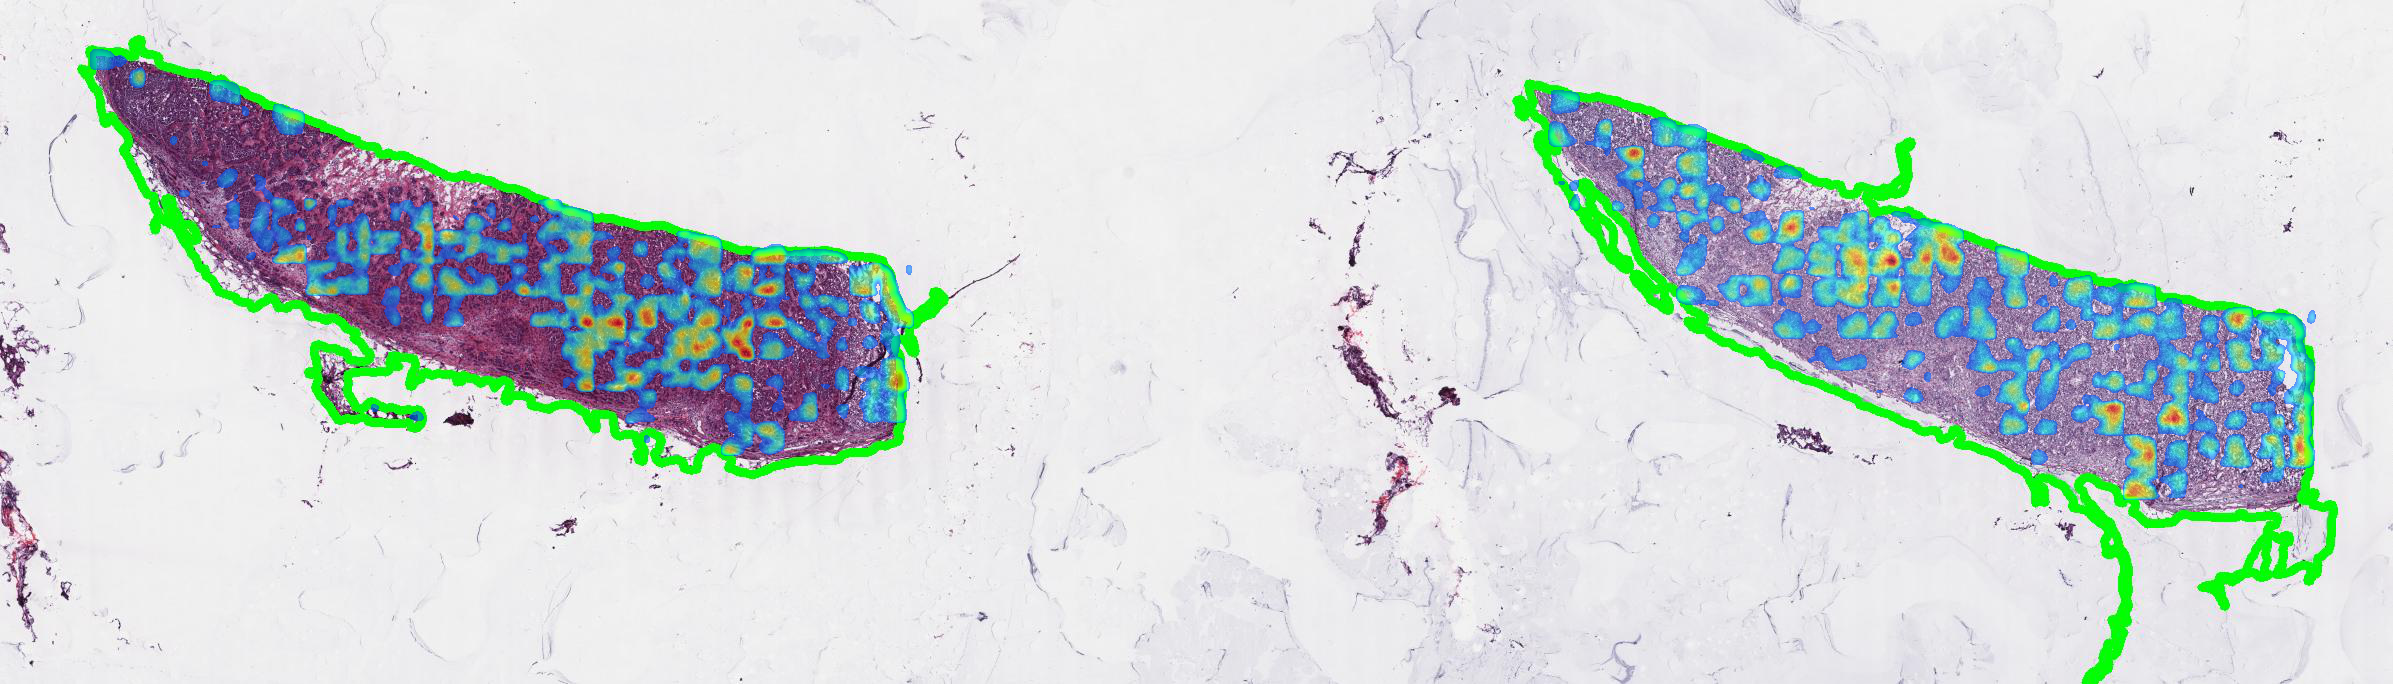
\includegraphics[width=1\textwidth]{images/attention_map_val.png}
	\caption{Final result that takes into account patch-level attention and inner patch features}
\end{figure}

\newpage

\section{Conclusions}


\end{document}